\documentclass[12pt]{article}
 \author{zhuangyz1998}   
 \title{papertitle} 
 \usepackage[pdftex]{graphicx}
 \usepackage{amsmath,amssymb}
 %\usepackage [doublespacing]{setspace}
 %\renewcommand{\baselinestrech}{1.5}
 \usepackage{fancyhdr}
 \pagestyle{fancy}
 \usepackage{lastpage}
 \lhead{Team \# 3211}
 \rhead{Page \thepage{} of \pageref{LastPage}}
 \cfoot{}
\begin{document} 
\maketitle  new paper test\\% This is comment
\textbf{Hello World!}\\
I understand A, B, C, \ldots, Z\\
The following text
\begin{center}
is centered.
\end{center}
\begin{verbatim}
\usepackage{textcomp}
\end{verbatim}

\tableofcontents

\section{Introduction}
\subsection{Restatement of the problem}
$$ \sum_{k=1}^n k = \frac{n(n+1)}{2} $$
$f(x)$ is equals to $\sin(x)$ and $\alpha$

\subsection{Random thoughts}
The equations
$\sum_{k=1}^3 \frac{1}{2} = \frac{7}{8}$
\begin{equation}
\sum_{k=1}^3 \frac{1}{2} = \frac{7}{8}
\end{equation}
and
\begin{equation*}
\sum_{k=1}^3 \frac{1}{2} = \frac{7}{8} \text{ for all real } x
\end{equation*}

\section{Conclusion}

The circle in Figure \ref{meterial} looks like a face.
\begin{figure}
\centering
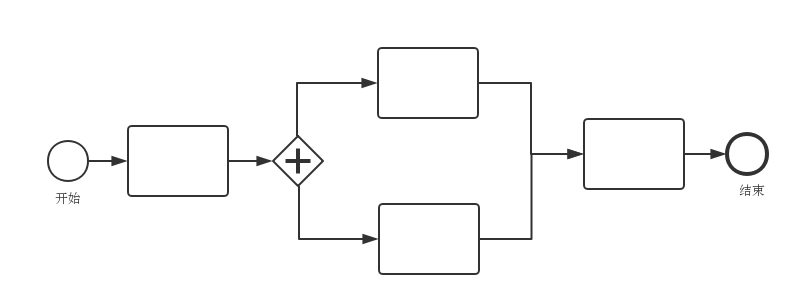
\includegraphics[width = 10cm]{meterial.png}
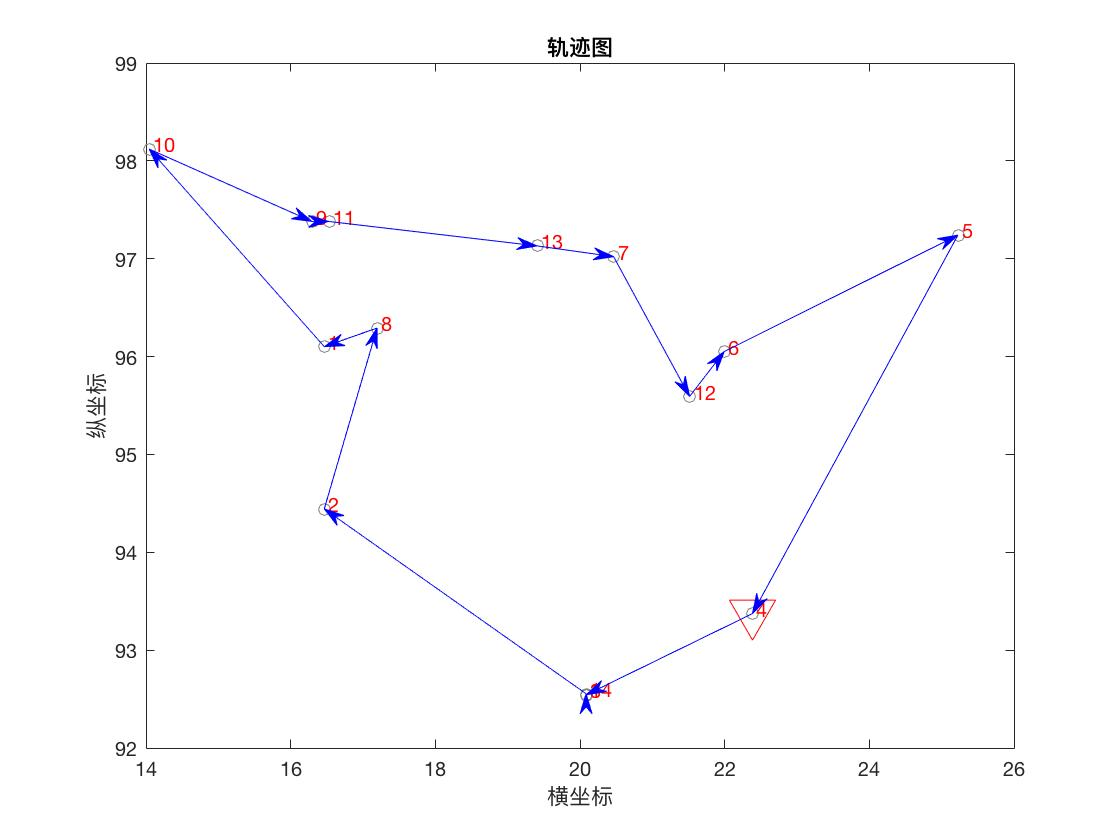
\includegraphics[width = 10cm]{graph.jpg}
\caption{This looks like UML.}
\label{meterial}
\end{figure}
\begin{align}
a + b &= c\\
	d &= e + f \nonumber\\
g + h &= i
\end{align}

\begin{align*}
a + b &= c\\
	d &= e + f \nonumber\\
g + h &= i
\end{align*}

\begin{equation*}
\begin{pmatrix}
1 & 2\\
3 & 4
\end{pmatrix}
\begin{bmatrix}
1 & 2\\
3 & 4
\end{bmatrix}
\begin{vmatrix}
1 & 2\\
3 & 4
\end{vmatrix}
\end{equation*}

\begin{itemize}
\item First Item.
\item Second Item.
\end{itemize}

\begin{enumerate}
\item First Item.
	\begin{enumerate}
	\item First Subitem.
	\item Second Subitem.
	\end{enumerate}
\item Second Item.
\end{enumerate}

This is part of
a paper\footnote{This is a footnote.}

The first four letters of the alphabet are in Table \ref{alpha}.

\begin{table}
\centering
\begin{tabular}{|c|l|r|}
\hline
Centered & \multicolumn{2}{c|}{Spread out} \\
\hline
0 & 1 & 2\\
1 & $x$ & $x^2$\\
\hline
\end{tabular}
\caption{Some Letters.}
\label{alpha}
\end{table}

It was shown in \cite{Te} that termites eat wood.


\begin{thebibliography}{99}
\bibitem{Carp}
Carpentwe, Bob.  \textsl{The Life of Ants.}
Springer-Verlag, Berlin, 1994.

\bibitem{Te}
Terwilliger, Sam.  \textsl{Termites.}
Prentice Hall, New York, 2004.
\end{thebibliography}
\end{document}